%% Author: Mohammed Hamza
%% Date:
%% Description: 
%% URL:

\documentclass[12pt,a4paper]{report}
\usepackage[left=1.5in, right=1.0in, top=1.0in, bottom=1.0in]{geometry}

% Check if with latex or pdflatex.
\ifx\pdftexversion\undefined
  \usepackage[dvips]{graphicx}
\else
  \usepackage[pdftex]{graphicx}
\fi

\usepackage{setspace}
\usepackage{titlesec}
\usepackage{enumerate}
\usepackage{enumitem}
\usepackage{amsmath}
\usepackage{amssymb}
\usepackage{fancyvrb}
\usepackage{float}
\usepackage{hyperref}
\usepackage{svg}
\usepackage{fancyhdr} % Required for fancy page styles
\usepackage{xcolor} % Required for defining custom colors
\usepackage{listings} % Required for code listings
\usepackage{tabulary}
\usepackage{multicol}
\usepackage{times}
\usepackage{epsfig}
\usepackage{tikz}
\usepackage{amsmath}
\usepackage{amsfonts}
\usepackage{listings}
\usepackage{amssymb}
\usepackage{booktabs}
\usepackage{tabularx}
\usepackage{circuitikz}
\usetikzlibrary{automata, positioning}
% \usepackage{sagetex}
% \usepackage{graphicx}
\usetikzlibrary{shapes, arrows.meta,arrows, positioning,chains, quotes}

% variables definition
\newcommand{\memberA}{Mohammed Hamza}
\newcommand{\indexA}{U03NM21T043044}

\newcommand{\guideA}{Professor Rithika Kannan}
% \newcommand{\guideB}{Dr HMV}
%auto-ignore
\renewcommand{\vec}[1]{\mathbf{#1}}

\usepackage{caption}
\usepackage{subcaption}
\usepackage{tabularx}
\usepackage{multirow}
\usepackage{amsmath}
\usepackage{tikz}
\usetikzlibrary{calc}
\usepackage{amssymb}
\usepackage{xcolor}
\usepackage{graphicx}
\usepackage{pgf}
\usepackage{pgfpages}
% \usepackage{background}
\usepackage{algorithm}% http://ctan.org/pkg/algorithms
%\usepackage{algpseudocode}% http://ctan.org/pkg/algorithmicx
\usepackage{algpseudocode}



\usepackage{amsthm}           
\newtheorem{thm}{Theorem}[section]
\newtheorem{lem}[thm]{Lemma}
\newtheorem{prop}[thm]{Proposition}
\newtheorem{cor}[thm]{Corollary}
\newtheorem{conj}[thm]{Conjecture}
\newtheorem{mydef}[thm]{Definition}

\renewcommand{\vec}[1]{\mathbf{#1}}

\newcommand{\Pro}{\operatorname{Pr_0}}
\newcommand{\X}{\mathbf{X}}
\newcommand{\Y}{\mathbf{Y}}
\newcommand{\Z}{\mathbf{Z}}
\newcommand{\I}{\mathbf{I}}
\newcommand{\Ninst}{N\operatorname{inst}}
\newcommand{\inst}{\texttt{inst}}
\newcommand{\x}{\vec{x}}
\newcommand{\y}{\vec{y}}
\newcommand{\z}{\vec{z}}
\newcommand{\Lstuff}{\mathcal{L}_{\operatorname{stuff}}}
\newcommand{\Lthings}{\mathcal{L}_{\operatorname{things}}}


\newcommand{\Sim}{\operatorname{Sim}}


\newcommand{\zo}{\vec{z}_1}
\newcommand{\zt}{\vec{z}_2}
\newcommand{\Cm}{\mathbb{C}^m}

\newcommand{\mylist}[1]{\begin{enumerate}#1\end{enumerate}}
  
\newcommand{\bd}[1]{\textbf{#1}}
\newcommand{\imI}{\mathrm{i}}

\newcommand{\indemp}[1]{\index{#1}\emph{#1}}

\newcommand{\minuseq}{\mathrel{{-}{=}}}
\newcommand{\pluseq}{\mathrel{{+}{=}}}
\newcommand{\coleq}{\mathrel{{:}{=}}}
\newcommand{\cl}{\operatorname{class}}
\newcommand{\addborder}{
    
\begin{tikzpicture}[remember picture, overlay]
        \draw[line width=1pt] 
            ($(current page.north west)+(0.5in,-0.5in)$) 
            rectangle 
            ($(current page.south east)+(-0.5in,1in)$);
    \end{tikzpicture}
}
\newcommand{\addborderb}{
    \begin{tikzpicture}[remember picture, overlay]
        \draw[line width=1pt] 
            ($(current page.north west)+(0.5in,-0.5in)$) 
            rectangle 
            ($(current page.south east)+(-0.5in,0.8in)$);
    \end{tikzpicture}
}

%\newcommand*\Let[2]{\State #1 $\gets$ #2}
%\algrenewcommand\alglinenumber[1]{
%    {\sf\footnotesize\addfontfeatures{Colour=888888,Numbers=Monospaced}#1}}
%\algrenewcommand\algorithmicrequire{\textbf{Precondition:}}
%\algrenewcommand\algorithmicensure{\textbf{Postcondition:}}

% Table of contents.
% \setcounter{secnumdepth}{3}
% \setcounter{tocdepth}{3}
% % Chapter title format, section format, subsection format.
% \titleformat{\chapter}
%   {\normalfont\Large\bfseries}{\thechapter}{1em}{}
% \titleformat{\section}
%   {\normalfont\Large\bfseries}{\thesection}{1em}{}
% \titleformat{\subsection}
%   {\normalfont\bfseries}{\thesubsection}{1em}{}
% 
% \titleformat{\section}[block]{\centering\Large\bfseries}{}{0pt}{} 
% \titlespacing*{\section}{0pt}{\baselineskip}{\baselineskip}
% % Chapter, section, subsection title spacings.
% \titlespacing*{\chapter}{0pt}{0ex plus 1ex minus .2ex}{2.3ex plus .2ex}
% \titlespacing*{\section} {0pt}{1ex plus 1ex minus .2ex}{1.5ex plus .2ex}
% \titlespacing*{\subsection} {0pt}{2ex plus 1ex minus .2ex}{1ex plus .2ex}

% renew counter for section numbering


% Spacing after a caption.
\setlength{\belowcaptionskip}{-15pt}

% % Spacing before a footer.
% \setlength{\skip\footins}{0.5cm}
\geometry{a4paper, margin=1in} 

\pagestyle{fancy}
\fancyhf{}
\fancyhead[L]{PLL implementation}


\pagestyle{fancy}
\fancyhf{} % Clear all header and footer fields
\fancyhead[L]{Transistor Level Implementation of PLL}
\fancyhead[R]{\makebox[\textwidth][r]{\textbf{\nouppercase{\leftmark}}}} % Right-alig

\fancyfoot[L]{\textbf{Department of ECE}} % Left side: Department name
\fancyfoot[C]{\textbf{Jan 2025 – Apr 2025}} % Center: Semester dates
\fancyfoot[R]{\textbf{Page \thepage}} % Right side: Page number
\renewcommand{\footrulewidth}{0.4pt}
% Define a custom page style for section pages
\fancypagestyle{chapterstyle}{
  \fancyhf{} % Clear all header and footer fields
  \renewcommand{\headrulewidth}{0pt} 
  \fancyfoot[L]{\textbf{Department of Electronics and Communication, UVCE}}% Left side: Department name
  \fancyfoot[C]{\textbf{Jan 2025 – Apr 2025}} % Center: Semester dates
  \fancyfoot[R]{\textbf{Page \thepage}} % Right side: Page number
}

% Apply custom style to section pages
% \makeatletter
% \preto\section{\thispagestyle{sectionstyle}}
% \makeatother

% \makeatletter
% \preto\chapter{\thispagestyle{chapterstyle}}
% \makeatother

% No header on the first page of a section




% \renewcommand{\section}{
%     \clearpage % Start each section on a new page
%     \pagestyle{plain} % Remove header
%     \oldsection
%     \thispagestyle{plain} % Ensure no header on this first page
%     \pagestyle{fancy} % Resume normal header style
% } have to check thisfkdljal;dskfa;sdkl;falsd;f

\definecolor{light-gray}{gray}{0.95} % Define the light-gray color
\lstset{
  basicstyle=\ttfamily\small,
  basicstyle=\ttfamily\small,
  keywordstyle=\color{blue}\bfseries,
  stringstyle=\color{red},
  commentstyle=\color{gray},
  morekeywords={int, return, Serial, if, else}, % Add any other keywords specific to your code
  numbers=left,
  numberstyle=\tiny\color{gray},
  stepnumber=1,
  breaklines=true,
  captionpos=b,
  tabsize=2,
  showspaces=false,
  showstringspaces=false,
  showtabs=false,
  breakatwhitespace=true,
  backgroundcolor=\color{light-gray}, % Set background color
}


\begin{document}
% \backgroundsetup{
%   scale=1,
%   color=black!20,
%   opacity=0.5,
%   angle=0,
%   position=current page.south,
%   vshift=10cm,
%   contents={
\includegraphics[width=0.7*\linewidth]{figs/university_logo.png}}
% }
% \pagestyle{empty}
\pagenumbering{roman}
  \onehalfspacing
  \begin{titlepage}

  \vspace{1 in}
  \begin{center}
  \newcommand*{\titlegroup}{
    \centering
    \vspace*{\baselineskip} % White space at the top of the page
	
	\rule{\textwidth}{1.6pt}\vspace*{-\baselineskip}\vspace*{2pt} % Thick horizontal line
	\rule{\textwidth}{0.4pt}\\[\baselineskip] % Thin horizontal line
	{\LARGE Data Converters In VLSI Systems} \\
	
	\rule{\textwidth}{0.4pt}\vspace*{-\baselineskip}\vspace{3.2pt} % Thin horizontal line
	\rule{\textwidth}{1.6pt}\\[\baselineskip] % Thick horizontal line
	
	\scshape % Small caps
	
	\vspace*{1\baselineskip} % Whitespace between location/year and editors
	{\large{\textsl{
				{A \\ 
					  Project Report \\ %\underline{•}
					Submitted in Partial Fulfillment of the Bangalore University\\
					for the Degree \\ 
					of\\
					\large \bf Bachelor of Technology \\
                    in\\
                    \large \bf Electronics and \\
                    \large \bf Communication Engineering 
	}}}}\\
	[5ex] \emph{by} \\[1ex]
	Submitted by \\[\baselineskip]
  \begin{tabular}{l l}
    \memberA & \indexA \\
  \end{tabular}
  }

  \titlegroup

  
\includegraphics[width=0.4\textwidth]{figs/university_logo.png} \\[1cm]

  \textbf{Department of Electronics and Communication Engineering} \\[0.2cm]
  \textbf{University of Visvesvaraya College of Engineering} \\[0.2cm]
  \textbf{K.R. Circle, Bangalore – 560 001} \\[0.2cm]
  \textbf{JUNE 2025}
    % \vspace{1.5 in}
    % \vspace{50mm}
    
    % \begin{flushleft}
    % \begin{multicols}{2}
    % 	Supervisors: \\
    % 	\guideA \\
    % 	\guideB \\
    % 	\vfill\null
    % 	\columnbreak
    	
    % 	Group Members: \\
    % 	\memberA \ (\indexA) \\
    % 	\memberB \ (\indexB) \\
    % 	\memberC \ (\indexC) \\
    % 	\memberD \ (\indexD) \\
    	

    % \end{multicols}
    % \end{flushleft}
    
%	Supervisor:	 	\hfill  	Group Members: \\
%    \guideA \hfill 	\memberA  - \indexA \\
%    \guideB \hfill 	\memberB  - \indexB \\
%    					  \hfill 	 \memberC  - \indexC \\
%   						  \hfill 	 \memberD  - \indexD \\
    

  \end{center}
\end{titlepage}


  \singlespacing
  
    % Roman numeral numbering until introduction.
  
  % \chapter*{Dedication}
% \addcontentsline{toc}{chapter}{Dedication}
\thispagestyle{empty}
\begin{center}
	\vfill
	To our families, friends, guide, and all others who supported us throughout this project.\\
	\vfill
\end{center}


  \pagestyle{plain}

  \pagenumbering{arabic}
  
  % \begin{flushleft}
\large{
	Approval of the Department of Electronic \& Telecommunication Engineering \\
}
	
  \vspace{30mm}

  \normalsize
\begin{multicols}{2}
	\vfill\null
	\columnbreak
	\begin{center}

		{\makebox[7cm]{\dotfill}} \\ 
		Head, Department of Electronic \& \\
		Telecommunication Engineering
 \\
	\end{center}
\end{multicols}


  \vspace{20mm}

This is to certify that I/we have read this project and that in my/our opinion it is fully adequate, in scope and quality, as an Undergraduate Graduation Project. \\

  \vspace{10mm}
  
  Supervisor: \guideA \\
    \vspace{15mm}
  Signature:  {\makebox[7cm]{\dotfill}}
\\
    \vspace{10mm}
  Date: {\makebox[7.9cm]{\dotfill}}
\\

\end{flushleft}

  % \chapter*{Declaration}
 \addcontentsline{toc}{chapter}{Declaration}  


\begin{flushleft}
	This declaration is made on February 15, 2020. \\
	\vspace{10mm}
	\textbf{Declaration by Project Group} \\
	We declare that the dissertation entitled Project Name and the work presented in it are our own. We confirm that:
	
	\begin{itemize}[noitemsep,topsep=0pt]
		\item this work was done wholly or mainly in candidature for a B.Sc. Engineering degree at this university,
		\item where any part of this dissertation has previously been submitted for a degree or any other qualification at this university or any other institute, has been clearly stated,
		\item where we have consulted the published work of others, is always clearly attributed,
		\item where we have quoted from the work of others, the source is always given,
		\item with the exception of such quotations, this dissertation is entirely our own work,
		\item we have acknowledged all main sources of help,
		\item parts of this dissertation have been published. (see \hyperref[chapter:appendix3]{List of Publications})
	\end{itemize}

\vspace{15mm}
\begin{multicols}{2}
	{\makebox[3cm]{\dotfill}} \\ 
	Date
	\vfill\null
	\columnbreak
	
	{\makebox[7cm]{\dotfill}} \\ 
	\memberA \  (\indexA)  \\
	\vspace{12mm}
	{\makebox[7cm]{\dotfill}} \\ 
	\memberB \ (\indexB)  \\
	\vspace{12mm}
	{\makebox[7cm]{\dotfill}} \\ 
	\memberC \ (\indexC)  \\
	\vspace{12mm}
	{\makebox[7cm]{\dotfill}} \\ 
	\memberD \ (\indexD)  \\

\end{multicols}


\end{flushleft}

  % \chapter*{Declaration by Supervisor}
 \addcontentsline{toc}{chapter}{Declaration by Supervisor}

\begin{flushleft}
	I/We have supervised and accepted this dissertation for the submission of the degree. \\

	\vspace{15mm}
	
	{\makebox[6.5cm]{\dotfill}} \hfill {\makebox[5cm]{\dotfill}}  \\ 
	\guideA \hfill Date \\
	
	
	\vspace{15mm}
	
	{\makebox[6.5cm]{\dotfill}} \hfill {\makebox[5cm]{\dotfill}}  \\ 
	\guideB \hfill Date \\
	
\end{flushleft}
 
  \chapter*{Abstract}
\addcontentsline{toc}{chapter}{Abstract}
% \begin{tikzpicture}[remember picture, overlay]
% 	% Draw border
% 	\draw[line width=0.5mm, color=black!20] (current page.south west) rectangle (current page.north east);
% 	% Add watermark text
% 	\node[rotate=45, scale=8, color=black!10, opacity=0.2] at (current page.center) {Mohammed Hamza};
% \end{tikzpicture}

\addborder
\begin{center}
	\vspace{5mm}
	\MakeUppercase{\textbf{DATA CONVERTERS IN VLSI SYSTEMS}}\\
	\vspace{5mm}
	% \memberA \\
	\vspace{5mm}
	% Guide: \guideA \\
	\vspace{5mm}
\end{center}

\noindent \textbf{Keywords:}\\
Data Converters, VLSI Systems, Analog-to-Digital Converter (ADC), Digital-to-Analog Converter (DAC), Successive Approximation Register (SAR), Sigma-Delta ADC, Signal Processing, Electronic Systems.
\\

In this report, we endeavor to understand Data Converters in VLSI Systems, 
focusing on the theoretical aspects of the Analog-to-Digital Converter (ADC) and Digital-to-Analog Converter (DAC).
We explore the principles of operation, design considerations, and performance metrics of these converters.
The report also delves into the different architecture of ADCs and DACs,
including their working principles, advantages, and disadvantages.
We discuss the various types of ADCs, such as Successive Approximation Register (SAR)
and Sigma-Delta ADCs, and the different types of DACs, including R-2R Ladder DACs and Current Steering DACs.
The report provides a comprehensive overview of the design and implementation of data converters in VLSI systems.The report highlights the importance of data converters in bridging the gap between analog and digital domains.enabling efficient signal processing and communication in electronic systems.The report is structured to provide transistor level implementation of Circuits in DACs and ADCs.

  \chapter*{Acknowledgements}
\addcontentsline{toc}{chapter}{Acknowledgements}
\addborder
\vspace{10mm}

\setstretch{1.5} We sincerely express our gratitude to our guide, \textbf{\guideA}, for her invaluable guidance, support, and encouragement throughout this project. We would also extend our gratitude towards Our Department's Esteemed HoD \textbf{Dr. Kiran K}. We are thankful to the Department of Electronics and Communication Engineering, UVCE, for providing us with the resources and opportunity to work on this project. Special thanks to our peers and family for their continuous motivation and assistance. We would also like to acknowledge the support of the administrative staff, whose help ensured smooth progress of our work. Additionally, we are grateful to the authors and researchers whose work has significantly contributed to our understanding and implementation. Finally, we recognize the inspiration and insights gained from discussions and feedback provided by our friends and colleagues. 


  
  \onehalfspacing
  \tableofcontents
  \addcontentsline{toc}{chapter}{Contents}
  \pagebreak
  
  \listoffigures
  \pagebreak
  
  \listoftables
  \pagebreak
  
    \chapter*{Abbreviations}
\addcontentsline{toc}{chapter}{Abbreviations}
\vspace{5mm}
\begin{tabular}{ll}
\textbf{ADC}  & Analog to Digital Converter \\
\textbf{DAC}  & Digital to Analog Converter \\
\textbf{SNR}  & Signal to Noise Ratio \\
\textbf{ENOB} & Effective Number of Bits \\
\textbf{INL}  & Integral Nonlinearity \\
\textbf{DNL}  & Differential Nonlinearity \\
\textbf{LSB}  & Least Significant Bit \\
\textbf{MSB}  & Most Significant Bit \\
\textbf{SAR}  & Successive Approximation Register \\
\textbf{T/H}  & Track and Hold \\
\textbf{S/H}  & Sample and Hold \\
\textbf{R-2R} & Resistor Ladder \\
\textbf{FS}   & Full Scale \\
\textbf{VLSI} & Very Large Scale Integration \\
\textbf{CMOS} & Complementary Metal-Oxide-Semiconductor \\
\end{tabular}

    % \chapter*{Symbols}
\addcontentsline{toc}{chapter}{Symbols}
\vspace{5mm}
\begin{tabular}{ll}
\textbf{C}    & Capacitance \\
\textbf{R}    & Resistance \\
\textbf{W}    & Width \\
\textbf{L}    & Channel length \\
\textbf{L}    & Inductor \\
\textbf{t}    & Time \\
\boldmath$\mu$ & Electron mobility \\
\textbf{C\textsubscript{ox}} & Oxide Capacitance \\
\textbf{V\textsubscript{ov}} & Voltage Overdrive \\
\boldmath$\phi$ & Phase \\
\boldmath$\zeta$ & Damping factor \\
\boldmath$\omega$ & Frequency in radians \\
\boldmath$\tau$ & Time constant \\
\end{tabular}
  

  % Change the numbering back to normal.
  \pagestyle{plain}
  \pagenumbering{arabic}
  \setcounter{page}{1}

  \onehalfspacing
  \pagestyle{fancy}
\fancyhf{}
\fancyhead[L]{PLL implementation}


\pagestyle{fancy}
\fancyhf{} % Clear all header and footer fields
\renewcommand{\headrulewidth}{1.5pt} 
% Define custom color for rules
\definecolor{myrulecolor}{RGB}{94,31,31}
\renewcommand{\headrule}{%
    {\color{myrulecolor}\hrule width\headwidth height\headrulewidth \vskip-\headrulewidth}
}
\fancyhead[L]{Data Converters In VLSI Systems} % Left-aligned header
\fancyhead[R]{\makebox[\textwidth][r]{\textbf{\nouppercase{\leftmark}}}} % Right-alig

\fancyfoot[L]{\textbf{Department of Electronics and Communication, UVCE}}
% \fancyfoot[C]{\textbf{Jan 2025 – Apr 2025}} % Center: Semester dates
\fancyfoot[R]{\textbf{Page \thepage}} % Right side: Page number
\renewcommand{\footrulewidth}{1.5pt}
\renewcommand{\footrule}{%
    {\color{myrulecolor}\hrule width\headwidth height\footrulewidth \vskip-\footrulewidth}
}
% Define a custom page style for section pages
\fancypagestyle{chapterstyle}{
        \fancyhf{} % Clear all header and footer fields
        \renewcommand{\headrulewidth}{0pt} 
        \fancyfoot[L]{\textbf{Department of ECE}} % Left side: Department name
%   \fancyfoot[C]{\textbf{Jan 2025 – Apr 2025}} % Center: Semester dates
        \fancyfoot[R]{\textbf{Page \thepage}} % Right side: Page number
}
\chapter{Introduction}
Data conveters are systems that convert analog signals to digital signals and digital signals to analog signals. These converters are termed as DACs (Digital to Analog Converters) and ADCs (Analog to Digital Converters). The
conversion of signals is essential in modern days as most of the systems are digital in nature. 
The conversion from Analog to Digital is majorly done by Quantizaion and Sampling. The quantization is the process of mapping a large set of input values to a smaller set of output values. The sampling is the process of converting a continuous signal into a discrete signal by taking samples at regular intervals.
The conversion from Digital to Analog is done by reconstructing the signal from the digital values. The reconstruction is done by using various techniques such as interpolation, filtering, etc
The figure \ref{fig:digital_analog_conversion} shows the conversion of digital signals to analog signals and vice versa. The digital signal are represented by discrete values, while the analog signals are represented by . 
\begin{figure}[H]
    \centering
    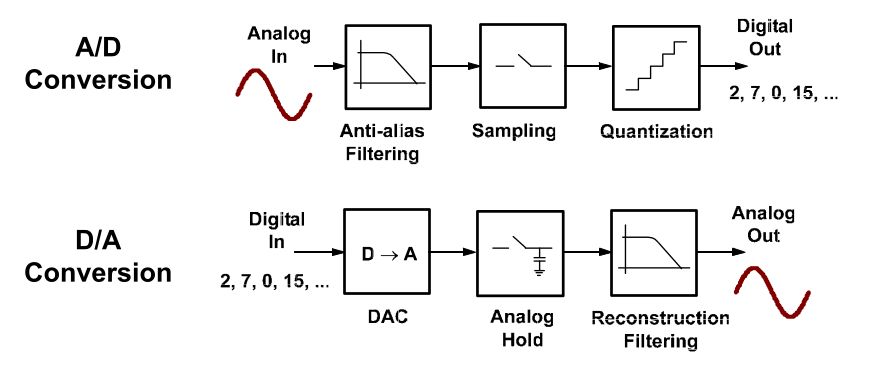
\includegraphics[width=0.8\textwidth]{figs/digital_and_analog_conversion.png}
    \caption{Digital and Analog Conversion}
    \label{fig:digital_analog_conversion}
\end{figure}
\section{Motivation}
Analog-to-Digital Converters (ADCs) and Digital-to-Analog Converters (DACs) provide a link between the Analog world and Digital world. They are essential as information is increalsingly being stored, processed, and transmitted in digital form. The need for high-performance ADCs and DACs is driven by the demand for high-speed data acquisition, signal processing, and communication systems.
physical systems are analog in nature, and the conversion of these signal helps in processing the signal in digital form hence we require D/A conversion interfaces.
Benifits of Digital signal processing
\begin{itemize}
    \item Reduced sensitivity to "analog" noise.
    \item Enhanced functionality and flexibility.
    \item Amenable to automated design \& test.
    \item Direct benefit from the scaling of VLSI technology.
\end{itemize}
\section{Brief History and DACs and ADCs}
Initially, Analog processing was done using analog circuits, but with the advent of digital technology Digital processing has become more prevalent. The first ADCs were developed in the 1950s and 1960s, and they were primarily used in military and aerospace applications. The first DACs were developed in the 1960s, and they were used in audio and video applications. Over the years, the technology has evolved, and today we have high-performance ADCs and DACs that are used in a wide range of applications, including telecommunications, consumer electronics, automotive, and industrial automation.

\section{Objective of the Report}
The objective of this report is to provide a comprehensive understanding of Data Converters in VLSI Systems, focusing on the theoretical aspects of Analog-to-Digital Converters (ADCs) and Digital-to-Analog Converters (DACs). The report aims to explore the principles of operation, design considerations, and performance metrics of these converters. It will also delve into the different CMOS circuits used in ADCs and DACs, including their working principles, advantages, and disadvantages. The report will
also explore research \& advancement Example. NeuADC- An automated design for ADC.


\section{Fundamentals of DACs and ADCs}
\subsection{Digital-to-Analog Converters (DACs)}
Digital-to-Analog Converters (DACs) perform the reverse operation of ADCs by converting discrete digital values into continuous analog signals. They reconstruct the analog signal from the digital input by generating a voltage or current that corresponds to the digital value. The resolution of a DAC is also determined by the number of bits used in the digital input. The performance of a DAC is characterized by parameters such as output voltage range, linearity, settling time, and noise performance.

\subsubsection{DACs Specifications}
The DAC converts an N-bit digital value into a continuous analog voltage, which is a scaled fraction of the reference voltage.
The output voltage (\(V_{out}\)) of a DAC can be expressed as:
\begin{equation}
    V_{out} = V_{REF} \cdot F
\end{equation}
where \(V_{\text{out}}\) is the analog voltage output, \(V_{\text{REF}}\) is the reference voltage, and \(F\) is the fraction defined by the input word, \(D\), that is \(N\) bits wide.
\begin{equation}
    Number\ of\ input\ conditions = 2^N
\end{equation}
F is the fraction of the reference voltage and corresponds to the digital input value \(D\) as follows:
\begin{equation}
    F = \frac{D}{2^N}
\end{equation}
\subsubsection{Specifications of DACs and ADCs}
\begin{itemize}
    \item \textbf{Differential Non-Linearity (DNL):} Measures the deviation of the step size between adjacent digital codes from the ideal value. A high DNL can cause missing codes and degrade performance.
    \item \textbf{Integral Non-Linearity (INL):} Represents the deviation of the actual transfer function from the ideal linear transfer function. It is a critical parameter for accuracy.
    \item \textbf{Offset:} Refers to the difference between the expected output and the actual output when the input is zero. It affects the accuracy of the converter.
    \item \textbf{Latency:} The time delay between the input signal and the corresponding output signal. Lower latency is essential for real-time applications.
    \item \textbf{Signal-to-Noise Ratio (SNR):} The ratio of the signal power to the noise power, indicating the quality of the conversion. Higher SNR values are desirable for better performance.
    \item \textbf{Dynamic Range:} The ratio between the largest and smallest signal levels that the converter can handle. A wide dynamic range is crucial for applications requiring high precision.
\end{itemize}
\subsection{Analog-to-Digital Converters (ADCs)}
Analog-to-Digital Converters (ADCs) are devices that convert continuous analog signals into discrete digital values. They sample the analog signal at regular intervals and quantize the sampled values into a finite number of levels. The resolution of an ADC is determined by the number of bits used to represent the digital output. For example, an 8-bit ADC can represent 256 discrete levels, while a 12-bit ADC can represent 4096 levels. The performance of an ADC is characterized by parameters such as sampling rate, resolution, signal-to-noise ratio (SNR), and total harmonic distortion (THD).
\subsubsection{ADCs Specifications}
DAC is converting a discrete
signal into an analog representation that is also limited by the resolution of the converter,
a fixed number of inputs and outputs are generated. However, with the ADC, the input is
an analog signal with an infinite number of values, which then has to be quantized into an
\(N\)-bit digital word
\begin{equation}
    Number\ of\ Quantizaion\ Levels = 2^N
\end{equation}

\subsection{Types of ADCs and DACs}
\subsubsection{Types of ADCs}
\begin{itemize}
    \item \textbf{Flash ADC:} Uses a resistor ladder network and comparators to convert analog signals to digital instantly. It is fast but consumes more power and area.
    \item \textbf{Successive Approximation Register (SAR) ADC:} Uses a binary search algorithm to approximate the input signal. It is widely used for medium-speed and medium-resolution applications.
    \item \textbf{Sigma-Delta ADC:} Utilizes oversampling and noise shaping to achieve high resolution. Commonly used in audio and precision measurement applications.
    \item \textbf{Pipeline ADC:} Combines multiple stages of ADCs to achieve high speed and resolution. Suitable for high-speed applications like video processing.
    \item \textbf{Dual-Slope ADC:} Measures the input signal by integrating it over a fixed period. It is slow but highly accurate, often used in digital multimeters.
\end{itemize}

\subsubsection{Types of DACs}
\begin{itemize}
    \item \textbf{Binary-Weighted DAC:} Uses resistors weighted in binary values to convert digital signals to analog. It is simple but requires precise resistor values.
    \item \textbf{R-2R Ladder DAC:} Employs a resistor ladder network for conversion. It is efficient and widely used due to its simplicity and scalability.
    \item \textbf{Current Steering DAC:} Converts digital signals to analog by steering currents through different paths. Commonly used in high-speed applications.
    \item \textbf{Sigma-Delta DAC:} Uses oversampling and noise shaping for high-resolution output. Suitable for audio applications.
    \item \textbf{Pulse Width Modulation (PWM) DAC:} Converts digital signals to analog by varying the duty cycle of a pulse. It is simple and cost-effective but requires filtering.
\end{itemize}

\section{Applications of Data Converters}
\begin{itemize}
    \item \textbf{Telecommunications:} Used in modems and communication systems to convert analog signals to digital for processing and vice versa.
    \item \textbf{Consumer Electronics:} Found in devices like smartphones, TVs, and audio systems for signal conversion and processing.
    \item \textbf{Automotive Systems:} Used in sensors and control systems for real-time data acquisition and processing.
    \item \textbf{Medical Devices:} Essential in imaging systems like MRI and CT scans for converting analog signals to digital for analysis.
    \item \textbf{Industrial Automation:} Used in control systems and sensors for monitoring and automation processes.
    \item \textbf{Aerospace and Defense:} Critical in radar systems, communication systems, and signal processing applications.
    \item \textbf{Instrumentation:} Used in digital oscilloscopes, multimeters, and other measurement devices for accurate data acquisition.
\end{itemize}

\subsection{Recent Advancements}


\subsection{issues and Challenges}
\begin{itemize}
    \item \textbf{Design Complexity:} Data converters are challenging to design due to the need for high precision and accuracy, especially with increasing performance requirements.
    \item \textbf{Performance Bottlenecks:} The speed, resolution, or power dissipation of ADCs and DACs can limit the overall system performance, making optimization critical.
    \item \textbf{Scaling Challenges:} As VLSI technology scales down, maintaining performance while reducing area and power consumption becomes increasingly difficult.
    \item \textbf{Noise and Distortion:} Minimizing noise and distortion in high-speed and high-resolution converters is a significant challenge.
    \item \textbf{Cost and Manufacturing Variability:} Achieving high performance while keeping costs low and addressing variability in manufacturing processes is a persistent issue.
\end{itemize}

  \chapter{Literature Review}
\addborderb
Data converters, primarily Analog-to-Digital Converters (ADCs) and Digital-to-Analog Converters (DACs), are essential components in modern electronic systems, enabling seamless interfacing between the analog real world and digital processing units. Over the past decades, significant advancements have been made in converter architectures, performance, and integration.

Early data converters were based on simple resistor ladder and integrating architectures, such as the successive approximation register (SAR) ADC and the binary-weighted DAC. These architectures offered moderate resolution and speed, suitable for early digital systems. As technology progressed, pipeline and sigma-delta (\(\Sigma\Delta\)) architectures emerged, providing higher resolution and faster conversion rates. Pipeline ADCs are widely used in applications requiring high speed and moderate resolution, such as communication systems, while sigma-delta converters excel in high-resolution, low-frequency applications like audio and instrumentation.

Recent literature has focused on improving the power efficiency, linearity, and area of data converters. Techniques such as calibration, digital correction, and time-interleaving have been proposed to overcome non-idealities and enhance performance. The scaling of CMOS technology has enabled the integration of high-performance data converters into system-on-chip (SoC) solutions, further driving research into low-voltage and low-power designs.

Emerging trends include the use of machine learning for calibration, the development of asynchronous and event-driven converters, and the exploration of new materials and device structures to push the boundaries of speed and resolution. The literature indicates a continuous trade-off between speed, resolution, power consumption, and area, with ongoing research aimed at optimizing these parameters for various application domains. 
  \chapter{Architeture of Data Converters}
\label{chapter:architecture}
\section{DAC Architecture}
\label{sec:dac_architecture}
DAC Architecture use varius techniques to convert digital signals to analog signals.
Some use voltage division, whereas others employ current
steering and even charge scaling to map the digital value into an analog quantity

\subsection{Resistor stringstyle DAC}
The resistor-string DAC, shown in Fig. \ref{fig:resistor_style}(a) uses 2N identical resistors and switches to divide voltage at selected taps, ensuring monotonic output. However, parasitic capacitance at the output node limits speed for higher resolutions. Fig. \ref{fig:resistor_style}(b) improves speed using a binary switch array, reducing the number of active switches. While compact designs are possible with active resistors, higher resolutions demand precise resistor values, balancing area and power dissipation.
The value of the output voltage is given by the equation \ref{eq:resistor_string_dac}
\begin{equation}
\label{eq:resistor_string_dac}
	V_{i,\text{ideal}} = \left( \frac{i V_{\text{REF}}}{2^N} \right), \quad \text{for } i = 0, 1, 2, \ldots, 2^N - 1
\end{equation}

\begin{center}
\begin{table}[H]
	\centering
	\label{tab:3bit_dac_output}
	\begin{tabular}{ccc|c}
		$D_2$ & $D_1$ & $D_0$ & $v_{\text{OUT}}$ \\
		\hline
		0 & 0 & 0 & 0 \\
		0 & 0 & 1 & 0.625 \\
		0 & 1 & 0 & 1.25 \\
		0 & 1 & 1 & 1.875 \\
		1 & 0 & 0 & 2.5 \\
		1 & 0 & 1 & 3.125 \\
		1 & 1 & 0 & 3.75 \\
		1 & 1 & 1 & 4.375 \\
	\end{tabular}
	\caption{Output voltages generated from the 3-bit DAC}
\end{table}
\end{center}
\begin{figure}[H]
	\centering
	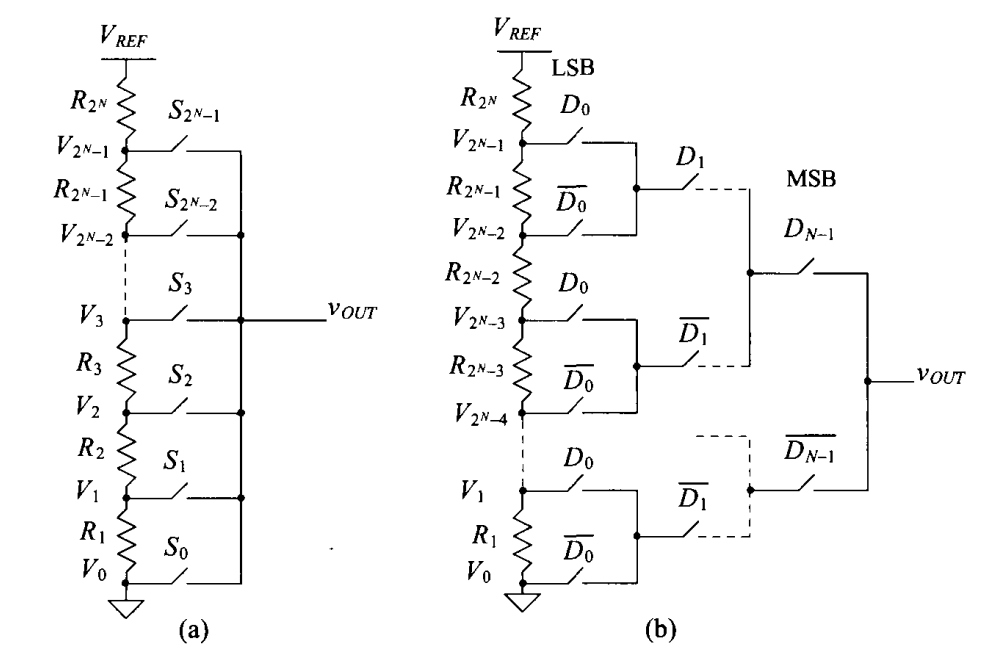
\includegraphics[width=0.7\textwidth]{figs/resistor_style.png}
	\caption{(a) A simple resistor-string DAC and (b) The use of a binary switch
array to lower the output capacitance}
	\label{fig:resistor_style}
	\vspace{0.5cm}
\end{figure}
\subsection{R-2R Ladder DAC}
The R-2R ladder DAC, shown in Fig. \ref{fig:r2r_dac}, employs a network of resistors alternating between values of R and 2R. This configuration ensures binary-weighted voltage division at each node, as illustrated in Fig. \ref{fig:r2r_dac}. The digital input switches each resistor to either ground or the inverting input of the op-amp, maintaining constant node voltages. The total current from the reference voltage remains constant, ensuring stable operation for varying digital inputs.
The output voltage, $v_{\text{OUT}}$, depends on currents flowing through the feedback resistor, $R_F$, such that
\begin{equation}
v_{\text{OUT}} = -i_{\text{TOT}} \cdot R_F \tag{29.14}
\end{equation}
where $i_{\text{TOT}}$ is the sum of the currents selected by the digital input, given by
\begin{equation}
i_{\text{TOT}} = \sum_{k=0}^{N-1} D_k \cdot \frac{V_{\text{REF}}}{2^{N-k}} \cdot \frac{1}{2R} \tag{29.15}
\end{equation}
where $D_k$ is the $k$-th bit of the input word with a value that is either a 1 or a 0.
\begin{figure}
	\centering
	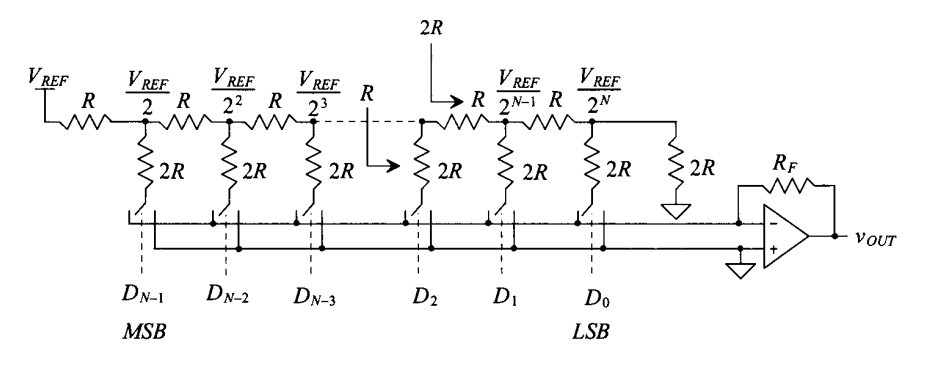
\includegraphics[width=0.7\textwidth]{figs/r2r_dac.png}
	\caption{A R-2R ladder digital-to-analog converter architecture}
	\label{fig:r2r_dac}
	\vspace{0.5cm}
\end{figure}
\subsection{Current Steering DAC}
Current steering DACs, shown in Fig. \ref{fig:current_steering_dac}, utilize a network of current sources to generate an output voltage proportional to the digital input rather then as in previous DAC where voltage was converted into current which generated voltage at the output. The current sources are controlled by switches that connect them to either the reference voltage or ground, allowing for precise control over the output current. This architecture is particularly effective for high-speed applications due to its fast switching capabilities and low output capacitance.
\begin{figure}
	\centering
	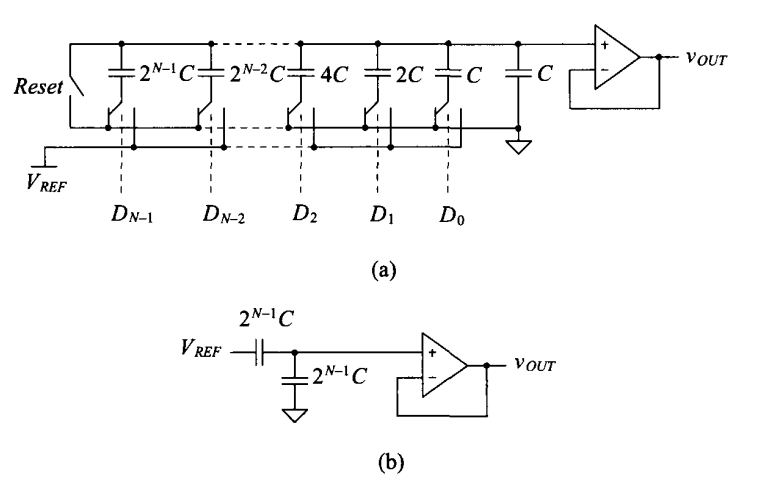
\includegraphics[width=0.7\textwidth]{figs/current_steering_dac.png}
	\caption{A current steering digital-to-analog converter architecture}
	\label{fig:current_steering_dac}
	\vspace{0.5cm}
\end{figure}
\subsection{Charge Scaling DAC}
The charge-scaling DAC, shown in Fig. \ref{fig:charge_scaling_dac}, employs a parallel array of binary-weighted capacitors connected to an op-amp. The capacitors are initially discharged, and the digital input switches each capacitor to either $V_{\text{REF}}$ or ground, creating an output voltage proportional to the digital input. This architecture is compact and efficient, making it suitable for applications requiring low power and high precision.

The output voltage, $v_{\text{OUT}}$, is given by:
\begin{equation}
v_{\text{OUT}} = \sum_{k=0}^{N-1} D_k \cdot 2^{k-N} \cdot V_{\text{REF}}
\end{equation}
where $D_k$ is the $k$-th bit of the digital input word, $V_{\text{REF}}$ is the reference voltage, and $N$ is the number of bits.

\begin{figure}[H]
	\centering
	\includegraphics[width=0.7\textwidth]{figs/charge_scaling_dac.png}
	\caption{(a) A charge-scaling DAC, (b) the equivalent circuit with the MSB = 1,and all other bits set to zero.}
	\label{fig:charge_scaling_dac}
	\vspace{0.5cm}
\end{figure}
\subsection{Cyclic DAC}
The cyclic DAC, shown in Fig. \ref{fig:cyclic_dac}, uses a minimal set of components to perform digital-to-analog conversion. It operates by processing one bit at a time in a serial fashion, requiring $N$ cycles for an $N$-bit conversion. The architecture employs a summer, a sample-and-hold (S/H) circuit, and an amplifier with a gain of 0.5. The summer adds $V_{\text{REF}}$ or ground to the feedback signal based on the input bits, while the amplifier feeds the output voltage back to the summer for the next cycle.

The output voltage at the end of the $n$-th cycle is given by:
\begin{equation}
v_{\text{OUT}}(n) = \left( D_{N-1} \cdot V_{\text{REF}} + \frac{1}{2} \cdot v_A(n-1) \right) \cdot \frac{1}{2}
\end{equation}
where $D_{N-1}$ is the most significant bit of the input word, $v_A(n-1)$ is the output voltage from the previous cycle, and $v_{\text{OUT}}(0)$ is initialized to zero.

This architecture is advantageous for its simplicity and ease of implementation using switched capacitors. However, its accuracy depends on the precision of the amplifier and the sample-and-hold circuit.

\begin{figure}[H]
	\centering
	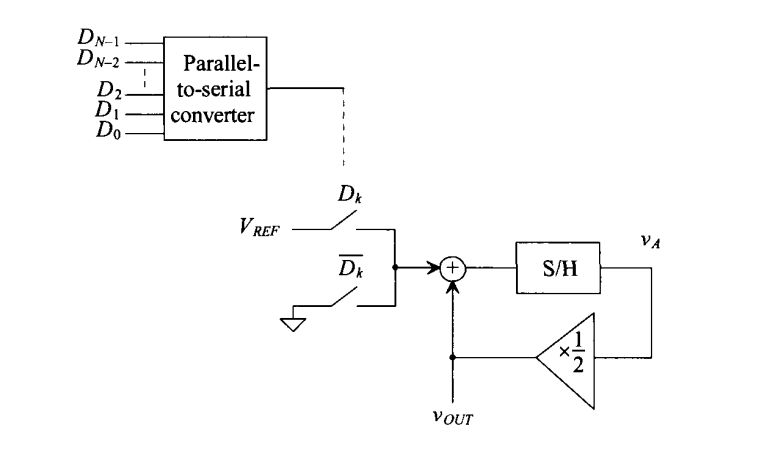
\includegraphics[width=0.7\textwidth]{figs/cyclic_dac.png}
	\caption{A cyclic digital-to-analog converter architecture}
	\label{fig:cyclic_dac}
	\vspace{0.5cm}
\end{figure}
\subsection{Pipline DAC}
The pipeline DAC, shown in Fig. \ref{fig:pipeline_dac}, extends the cyclic DAC architecture by employing multiple stages, each responsible for processing one bit of the digital input. This configuration allows for continuous operation, as each stage processes a new bit while passing the intermediate result to the next stage. The architecture consists of sample-and-hold (S/H) circuits, summers, and amplifiers with a gain of 0.5.

The output voltage at the $n$-th stage is given by:
\begin{equation}
v_{\text{OUT}}(n) = \left( D_{n-1} \cdot V_{\text{REF}} + v_{\text{OUT}}(n-1) \right) \cdot \frac{1}{2}
\end{equation}
where $D_{n-1}$ is the bit processed by the $n$-th stage, $v_{\text{OUT}}(n-1)$ is the output voltage from the previous stage, and $v_{\text{OUT}}(0)$ is initialized to zero.

This architecture is advantageous for its high throughput, as it produces one output per clock cycle after an initial delay of $N$ cycles. However, it requires precise amplifier gains and increased circuitry compared to cyclic DACs.

\begin{figure}[H]
	\centering
	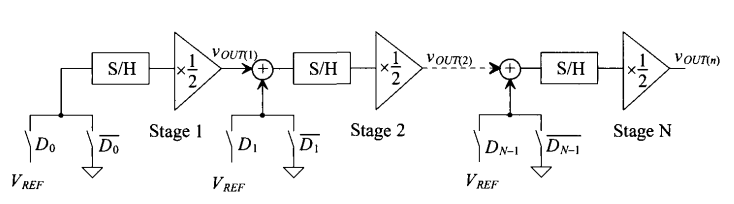
\includegraphics[width=0.7\textwidth]{figs/pipeline_dac.png}
	\caption{A pipeline digital-to-analog converter architecture}
	\label{fig:pipeline_dac}
	\vspace{0.5cm}
\end{figure}
\section{ADC Architecture}
\label{sec:adc_architecture}
ADC Architecture use various techniques to convert analog signals to digital signals.
Some use voltage division, whereas others employ current
steering and even charge scaling to map the analog value into a digital quantity.
\subsection{Flash ADC}
The flash ADC, shown in Fig. \ref{fig:flash_adc}, is the fastest type of ADC architecture. It uses a resistor-string DAC to divide the reference voltage into $2^N$ levels, where $N$ is the resolution of the ADC. Each level is fed into a comparator, which compares the input voltage with the reference levels and generates a thermometer code. The thermometer code is then converted into a binary digital output using a decoder.

The flash ADC requires $2^N - 1$ comparators and $2^N$ resistors, making it area-intensive for higher resolutions. However, its speed is unmatched, as it performs the conversion in a single clock cycle. The disadvantages of the flash ADC include high power consumption and increased complexity for higher resolutions.

\begin{figure}[H]
	\centering
	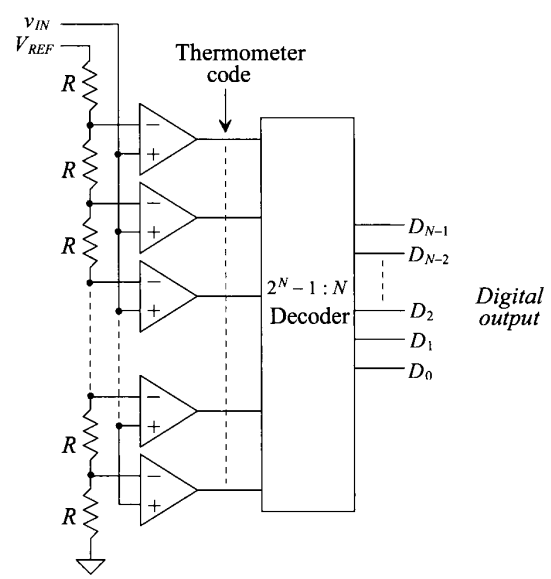
\includegraphics[width=0.7\textwidth]{figs/flash_adc.png}
	\caption{Block diagram of a Flash ADC architecture}
	\label{fig:flash_adc}
	\vspace{0.5cm}
\end{figure}
\subsection{Successive Approximation Register (SAR) ADC}
The successive approximation register (SAR) ADC, shown in Fig. \ref{fig:sar_adc}, performs analog-to-digital conversion using a binary search algorithm. It employs a sample-and-hold (S/H) circuit, a comparator, a digital-to-analog converter (DAC), and a successive approximation register (SAR). The SAR controls the DAC output based on the comparator's feedback, iteratively refining the digital output.

The conversion process begins by sampling the input voltage, $v_{\text{IN}}$, and initializing the SAR to its midpoint value. The comparator compares $v_{\text{IN}}$ with the DAC output, adjusting the SAR value accordingly. This process repeats for $N$ cycles, where $N$ is the resolution of the ADC, producing the final digital output.

The SAR ADC is advantageous for its balance between speed and power consumption, making it suitable for medium-speed applications. However, its accuracy depends on the precision of the DAC and comparator.

\begin{figure}[H]
	\centering
	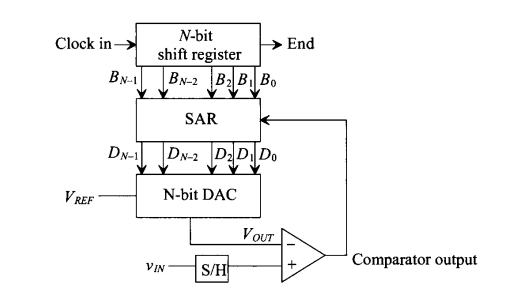
\includegraphics[width=0.8\textwidth]{figs/sar_adc.png}
	\caption{Block diagram of a Successive Approximation Register (SAR) ADC architecture}
	\label{fig:sar_adc}
	\vspace{0.5cm}
\end{figure}
\subsection{Pipeline ADC}
The pipeline ADC, as illustrated in Fig.~\ref{fig:pipeline_adc}, achieves high throughput by dividing the conversion process into multiple stages, each resolving a single bit (or a few bits) per stage. Each stage typically consists of a sample-and-hold (S/H) circuit, a 1-bit ADC (comparator), a digital-to-analog sub-converter (DAC), a subtractor, and a gain stage (usually by 2). The residue from each stage is passed to the next, allowing pipelined operation.

The operation of each stage is as follows:
\begin{enumerate}
	\item The input signal is sampled and compared to $\frac{V_{\text{REF}}}{2}$ by the 1-bit ADC.
	\item If $v_{\text{IN}} > \frac{V_{\text{REF}}}{2}$, the comparator outputs 1; otherwise, it outputs 0. The corresponding reference ($0$ or $\frac{V_{\text{REF}}}{2}$) is subtracted from the input to generate the residue.
	\item The residue is amplified by 2 and passed to the next stage.
\end{enumerate}

After an initial latency of $N$ clock cycles (for an $N$-stage pipeline), the converter outputs one result per clock cycle, making it suitable for high-speed applications. The main trade-offs are increased circuit complexity and the need for precise inter-stage gain and timing.

\begin{figure}[H]
	\centering
	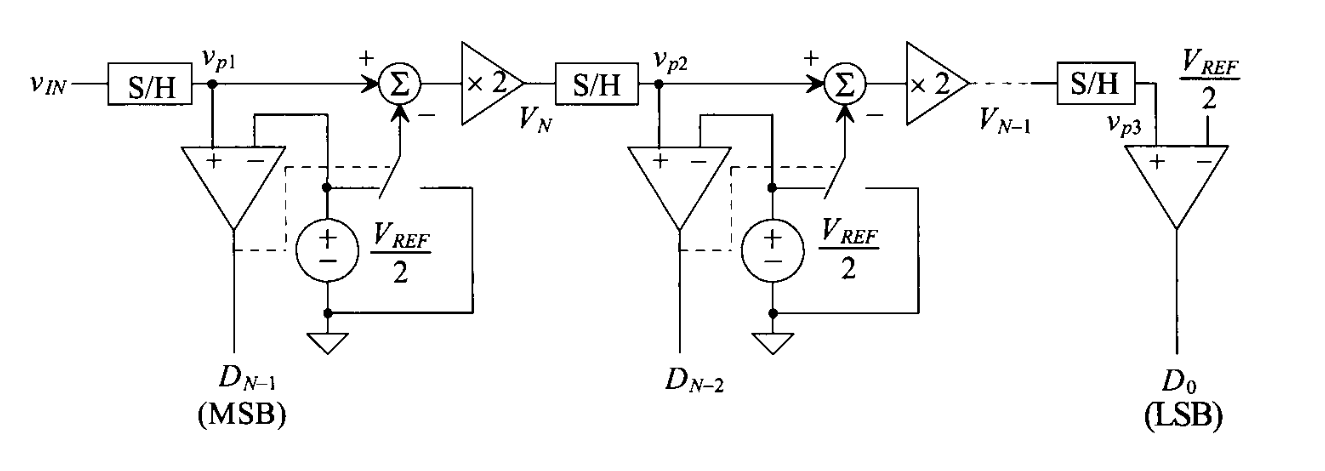
\includegraphics[width=0.8\textwidth]{figs/pipeline_adc.png}
	\caption{Block diagram of a pipeline ADC architecture}
	\label{fig:pipeline_adc}
	\vspace{0.5cm}
\end{figure}


  \chapter{Implementation of Data Converters}
\addborderb
\label{chapter:results}
\section{Sub-Circuits Used in Data Converters}

\subsection{Sample and Hold (S/H) Circuits}
Sample and hold (S/H) circuits or Amplifiers are required to sample the analog input signal and hold it during the full cycle of clock period give to the ADC.
\subsubsection{Basic S/H Topology}
\paragraph{Basic Configuration}
The basic sample-and-hold (S/H) circuit consists of an analog switch (typically implemented with a MOSFET) in series with a hold capacitor $C_H$. The input signal $V_{in}$ is sampled when the switch is closed, charging $C_H$ to $V_{in}$. When the switch opens, $C_H$ holds the sampled voltage, which can be read as $V_{out}$. The ON resistance $R_s$ of the switch and the value of $C_H$ determine the bandwidth and acquisition time of the circuit. The small-signal $-3$ dB bandwidth is given by:
\begin{equation}
    f_{-3\,\mathrm{dB}} = \frac{1}{2\pi R_s C_H}
\end{equation}
The acquisition time, i.e., the time required for $V_{out}$ to settle within a specified accuracy of $V_{in}$, is determined by the RC time constant. The basic configuration is shown in Figure~\ref{fig:basic_sh_config}.
\begin{figure}[h]
    \centering
    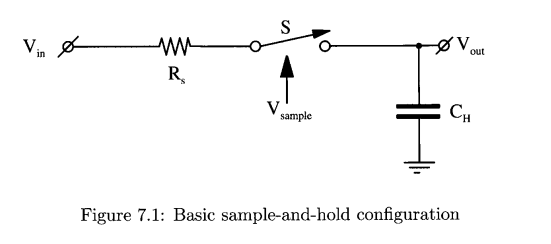
\includegraphics[width=0.5\textwidth]{figs/basic_sh_config.png}
    \caption{Basic Sample and Hold Circuit Configuration}
    \label{fig:basic_sh_config}
\end{figure}
by using a differential sample and hold circuit shown in Fig. \ref{fig}
the second order harmonic distortion can be avoided.
\begin{figure}
    \centering
    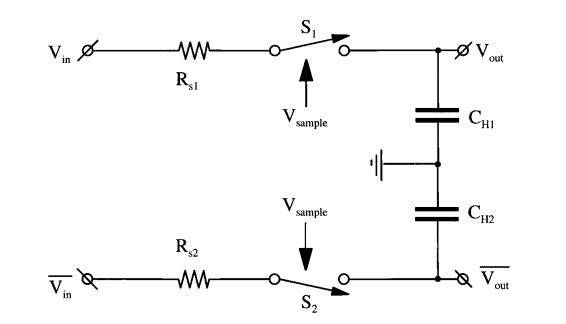
\includegraphics[width=0.7\textwidth]{figs/differential_sh.png}
    \caption{Differential Sample and Hold Circuit Configuration}
    \label{fig:differential_sh_config}
\end{figure}
\subsubsection{Integrated Sample and Hold Circuits}
Integrated sample-and-hold (S/H) circuits use operational amplifiers to improve accuracy, reduce charge injection, and provide buffering. A common topology is the integrating S/H circuit, as shown in Figure~\ref{fig:integrating_sh_circuit}. Here, the hold capacitor $C_H$ is connected between the output and the inverting input of an op-amp, forming an integrator. The analog switch $S$ samples the input signal onto $C_H$ when closed. When $S$ opens, the op-amp holds the voltage across $C_H$, providing a stable output.

\begin{figure}[h]
    \centering
    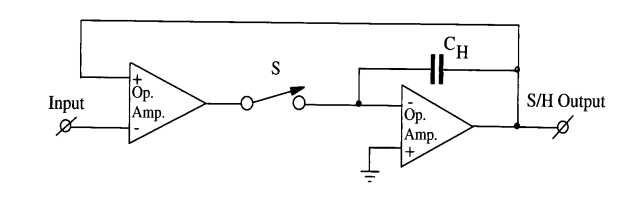
\includegraphics[width=0.7\textwidth]{figs/integrating_sh_config.png}
    \caption{Integrating sample-and-hold circuit}
    \label{fig:integrating_sh_circuit}
\end{figure}

This configuration minimizes the effects of charge injection and clock feedthrough by ensuring that the switch operates at a virtual ground. The op-amp buffer also isolates the hold capacitor from the load, improving hold accuracy. Special care must be taken in the design of the op-amp and switch to ensure low offset, high slew rate, and minimal leakage for precise sampling and holding.
\subsubsection{Practical integrated S/H circuit}
A practical example of an integrated sample-and-hold (S/H) circuit is shown in Figure~\ref{fig:practical_sh_circuit}. This circuit uses a differential input amplifier ($M_1$, $M_2$), loaded with a current mirror ($M_3$, $M_4$). The output current is integrated onto the hold capacitor $C_H$, which is connected between the drain and gate of the Miller stage transistor $M_6$. Biasing is provided by current source transistors $M_7$ and $M_8$, with their gates tied to a bias voltage $V_{bias}$. The sampling operation is controlled by switch $M_5$. During the track phase, $M_5$ is closed, allowing the output current to charge $C_H$ and track the input. When switched to hold mode, $M_5$ opens, and the voltage stored on $C_H$ is held, providing the output. This topology ensures low aperture uncertainty and minimizes the need for clock boosting circuits, as $M_5$ operates near the same gate-source voltage as $M_6$.

\begin{figure}[h]
    \centering
    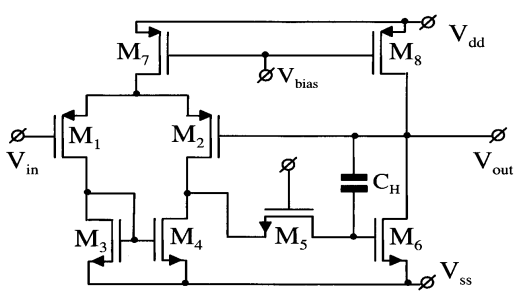
\includegraphics[width=0.7\textwidth]{figs/practical_sh_config.png}
    \caption{Integrated sample-and-hold circuit implementation}
    \label{fig:practical_sh_circuit}
\end{figure}

\subsection{Comparator Circuits}
Comparators are essential components in ADCs, used to compare the input signal with a reference voltage and produce a digital output indicating which is higher. They can be implemented using various techniques, each with its own advantages and trade-offs.
\begin{figure}[H]
    \centering
    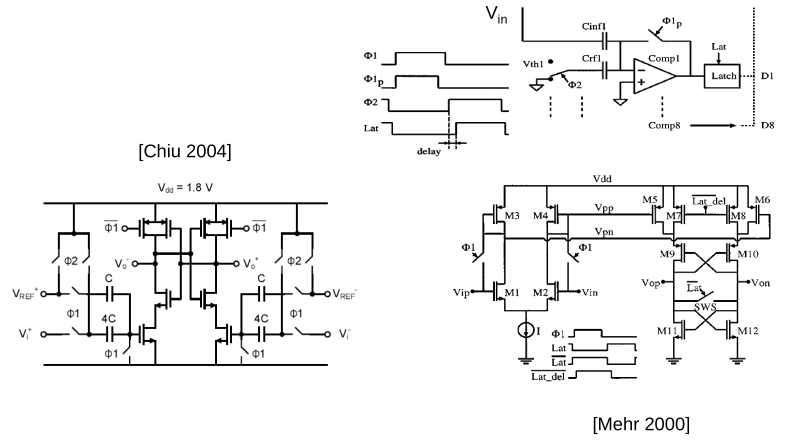
\includegraphics[width=0.7\textwidth]{figs/compartator_circuits.png}
    \caption{Few Comparator Circuits}
    \label{fig:comparator_circuit}
\end{figure}
\subsection{Digital-to-Analog Sub-Circuits}
\subsubsection{Binary-Weighted Current Source}
The binary-weighted current source DAC is a fundamental architecture that uses MOS transistors sized in binary ratios to generate output currents proportional to the digital input code. Each bit controls a current source whose value is weighted as a power of two, as shown in Figure~\ref{fig:binary_weighted_current_source}.

\begin{figure}[h]
    \centering
    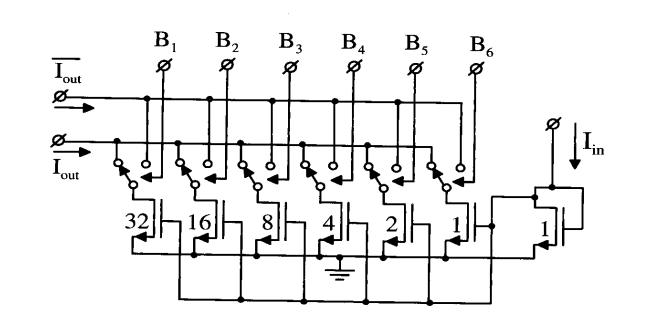
\includegraphics[width=0.8\textwidth]{figs/binary_weighted_current_source.png}
    \caption{MOS-only binary weighted current network}
    \label{fig:binary_weighted_current_source}
\end{figure}

In this structure, the reference current $I_{in}$ is mirrored and scaled by MOS transistors with widths proportional to $2^n$, where $n$ is the bit position. The output current $I_{out}$ is the sum of the selected currents, determined by the digital input bits $B_1$ to $B_N$:
\begin{equation}
    I_{out} = I_{ref} \sum_{k=0}^{N-1} b_k 2^k
\end{equation}
where $b_k$ is the $k$-th digital input bit.

\textbf{Advantages:}
\begin{itemize}
    \item Simple and fast operation.
    \item Direct current output, suitable for high-speed applications.
\end{itemize}

\textbf{Limitations:}
\begin{itemize}
    \item Requires precise current source matching and layout.
    \item Large area for high-resolution DACs due to exponential scaling of device sizes.
    \item Sensitive to channel length modulation and device mismatches.
\end{itemize}

\subsubsection{R-2R Ladder Network}
    The R-2R ladder network is a widely used architecture for implementing digital-to-analog converters (DACs) due to its simplicity, scalability, and ease of integration. It consists of resistors with only two values: $R$ and $2R$, arranged in a ladder-like structure. Each digital input bit controls a switch that connects the corresponding node either to a reference voltage or to ground, generating a binary-weighted output current or voltage.

    \begin{figure}[h]
        \centering
        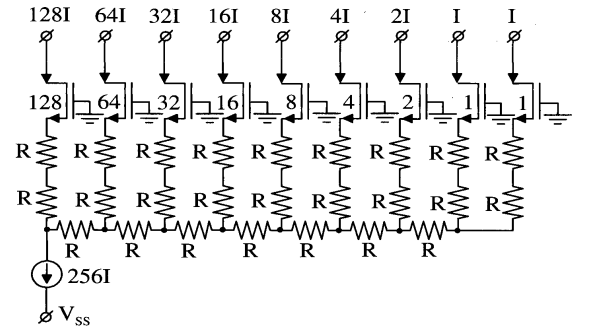
\includegraphics[width=0.85\textwidth]{figs/r2r_ladder.png}
        \caption{R-2R Ladder Network DAC Structure}
        \label{fig:r2r_ladder}
    \end{figure}

    The output voltage $V_{out}$ for an $N$-bit R-2R DAC can be expressed as:
    \begin{equation}
        V_{out} = V_{ref} \cdot \frac{1}{2^N} \sum_{k=0}^{N-1} b_k 2^{k}
    \end{equation}
    where $b_k$ is the $k$-th digital input bit (0 or 1), and $V_{ref}$ is the reference voltage.

    \textbf{Advantages:}
    \begin{itemize}
        \item Requires only two resistor values, simplifying layout and matching.
        \item Good linearity and monotonicity if resistor matching is precise.
        \item Easily scalable to higher resolutions.
    \end{itemize}

    \textbf{Design Considerations:}
    \begin{itemize}
        \item Resistor matching and layout are critical for accuracy.
        \item Output impedance and loading effects must be minimized.
        \item Parasitic capacitances can limit speed at high resolutions.
    \end{itemize}
    \subsubsection{MOS R-2R implementation}
    The MOS implementation of the R-2R ladder network replaces passive resistors with MOS transistors operating in the triode (linear) region, allowing for compact integration and process compatibility. Figure~\ref{fig:r2r_mos_elements} illustrates typical MOS-based R-2R cells and their possible configurations.

    \begin{figure}[h]
        \centering
        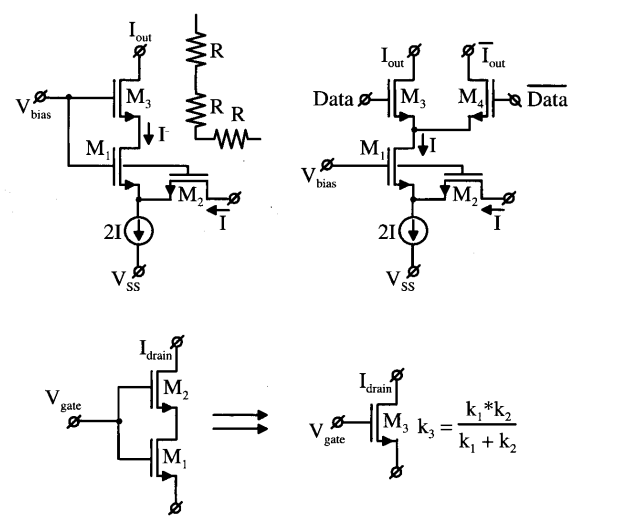
\includegraphics[width=0.85\textwidth]{figs/r2r_mos_elements.png}
        \caption{R-2R MOS elements: (a) Basic MOS R-2R cell, (b) Bit current switch integration, (c) Equivalent resistance using MOS transistors}
        \label{fig:r2r_mos_elements}
    \end{figure}

    In these circuits, matched MOSFETs ($M_1$, $M_2$, $M_3$, etc.) are biased such that their channel resistance emulates the required $R$ and $2R$ values. The current division and switching are achieved by controlling the gate voltages or digital data lines. When the MOSFETs operate in the triode region, their resistance is approximately:
    \begin{equation}
        R_{DS(on)} \approx \frac{1}{\mu_n C_{ox} \frac{W}{L} (V_{GS} - V_{th})}
    \end{equation}
    where $W/L$ is the transistor aspect ratio, $V_{GS}$ is the gate-source voltage, and $V_{th}$ is the threshold voltage.

    \textbf{Advantages:}
    \begin{itemize}
        \item Fully compatible with CMOS processes, enabling high integration.
        \item Area-efficient compared to passive resistor ladders.
        \item Programmable resistance by adjusting $W/L$ ratios or bias voltages.
    \end{itemize}

    \textbf{Limitations:}
    \begin{itemize}
        \item Non-idealities due to MOSFET mismatch, channel length modulation, and voltage dependence of $R_{DS(on)}$.
        \item Limited linearity and temperature stability compared to passive resistors.
        \item Careful biasing and layout are required for accurate operation.
    \end{itemize}

    This approach is especially useful in applications where integration density and process compatibility are prioritized over absolute accuracy.
\subsubsection{Capacitive DAC (CDAC)}
The capacitive digital-to-analog converter (CDAC) is a widely used architecture in CMOS technology due to its excellent matching properties, low power consumption, and ease of integration. The CDAC operates by redistributing charge among a binary-weighted array of capacitors, as shown in Fig. ~\ref{fig:binary_weighted_capacitor_dac}.

\begin{figure}[h]
    \centering
    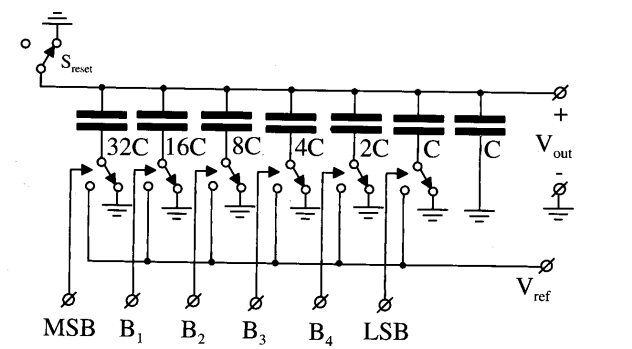
\includegraphics[width=0.85\textwidth]{figs/binary_weighted_capacitor_dac.png}
    \caption{Binary-weighted capacitor DAC structure}
    \label{fig:binary_weighted_capacitor_dac}
\end{figure}

\paragraph{Operation Principle}
The CDAC consists of $N$ binary-weighted capacitors ($C$, $2C$, $4C$, ..., $2^{N-1}C$) and a unit capacitor for charge balancing. Each capacitor can be switched between a reference voltage $V_{ref}$ and ground, depending on the digital input code. During operation, all capacitors are first discharged (reset phase). Then, based on the digital input, selected capacitors are connected to $V_{ref}$, while others remain at ground. The resulting output voltage is given by:
\begin{equation}
    V_{out} = \frac{V_{ref}}{2^N} \sum_{i=1}^{N} D_i \cdot 2^{i-1}
\end{equation}
where $D_i$ is the $i$-th digital input bit.

\paragraph{Advantages}
\begin{itemize}
    \item Excellent matching and linearity due to capacitor array.
    \item Low static power consumption.
    \item Fully compatible with CMOS processes.
\end{itemize}

\paragraph{Design Considerations}
\begin{itemize}
    \item Capacitor matching and layout symmetry are critical for accuracy.
    \item Parasitic capacitance and switch charge injection can affect performance.
    \item Output buffer is often required to prevent loading effects.
\end{itemize}

CDACs are commonly used in SAR ADCs and other mixed-signal systems where high linearity and integration are required.

% \subsection{Analog Multiplexers and Switches}
% \subsubsection{CMOS Transmission Gate}
% \subsubsection{Bootstrapped Switch}
% \subsubsection{On-resistance Variation and Signal Distortion}

% \subsection{Operational Amplifiers and Integrators}
% \subsubsection{Single-Stage and Two-Stage Op-Amps}
% \subsubsection{Miller Compensation}
% \subsubsection{OTA for Integrators in $\Sigma\Delta$ ADCs}
% OTAs are used in $\Sigma\Delta$ ADCs for integration and feedback.

% \subsection{Current Mirrors and Biasing Circuits}
% \subsubsection{Simple and Cascode Current Mirrors}
% \subsubsection{Bandgap Reference Circuits}
% \subsubsection{Biasing Techniques for Analog Blocks}

% \subsection{Timing and Control Logic (Brief Theoretical Overview)}
% \subsubsection{Clock Generation}
% \subsubsection{Control FSM for SAR Logic}
% \subsubsection{Latch Timing in Pipeline or Flash ADCs}

% \section{Summary}
% Interrelation of sub-circuits in ADC/DAC architectures.

% \section{Design Trade-offs}
% Speed vs power, accuracy vs area.

  \chapter{Conclusion \& Future Work}
\section{Conclusion}
This Report presents the Data Converters in VLSI Systems and make use of various techniques to implement the Data Converters. The report covers the architecture of ADC and DAC, their implementation, and the design considerations for low power and high performance. The report also discusses the challenges faced during the design process and how they were addressed.
Few primary subcircuits present in Data converters are presented in the report example S/H circuits, comparators, and etc. 
\section{Comparison of DAC \& ADC Architectures}
This section provides a comparative analysis of various DAC and ADC architectures, highlighting their advantages, disadvantages, and typical applications. The comparison is summarized in Tables \ref{tab:adc_comparison} and \ref{tab:dac_comparison}.
\begin{table}[h!]
\centering
\begin{tabular}{|p{2.8cm}|p{4cm}|p{4cm}|p{4cm}|}
\hline
\textbf{DAC Type} & \textbf{Advantages} & \textbf{Disadvantages} & \textbf{Typical Applications} \\
\hline
Resistor String & Simple design, monotonic & Large area for high resolution, slow & Low-cost, low-speed systems \\
\hline
R-2R Ladder & Compact, easy to scale & Sensitive to resistor mismatch & Audio, signal generation \\
\hline
Current Steering & High speed, good linearity & Complex layout, higher power & High-speed communications \\
\hline
Sigma-Delta & High resolution, noise shaping & Slow conversion rate, complex digital filter & Audio, instrumentation \\
\hline
\end{tabular}
\caption{Comparison of Different DAC Architectures}
\label{tab:dac_comparison}
\end{table}

\begin{table}[h!]
\centering
\begin{tabular}{|p{2.8cm}|p{3.5cm}|p{3.8cm}|p{3.2cm}|}
\hline
\textbf{ADC Type} & \textbf{Advantages} & \textbf{Disadvantages} & \textbf{Typical Applications} \\
\hline
Flash & Fast conversion, simple architecture & High power consumption, large area for high resolution & High-speed applications \\
\hline
Successive Approximation & Good speed-power trade-off, moderate complexity & Slower than flash, limited resolution & Medium-speed applications \\
\hline
Pipeline & High speed, good resolution & Complex design, requires precise components & High-speed data acquisition \\
\hline
Sigma-Delta & High resolution, noise shaping & Slow conversion rate, complex digital filter & Audio, instrumentation \\
\hline
\end{tabular}
\caption{Comparison of Different ADC Architectures}
\label{tab:adc_comparison}
\end{table}

\section{Future Work}
The future work includes the implementation of more advanced data converters with improved performance metrics such as higher resolution.Simulating the data converters using advanced simulation tools to validate the design and performance metrics. Additionally, exploring the use of machine learning techniques for optimizing the design and performance of data converters in VLSI systems. The report also suggests further research in the area of low power design techniques for data converters to enhance their efficiency and performance in modern electronic systems.


\nocite{bookpll}
\nocite{vandeplassche2003cmos}
\nocite{vandeplassche1988eightbit}
\nocite{abrial1988analog}
\nocite{schouwenaars1988lowpower}
\nocite{jin2014energyefficient}
\nocite{vandeplassche1982monolithic}

  % \singlespacing
    \addcontentsline{toc}{chapter}{References}
  \renewcommand{\bibname}{References}
  \bibliographystyle{IEEEtran}
  \bibliography{thesis}
  % \chapter*{\raggedleft Appendix A}
\addcontentsline{toc}{chapter}{Appendix A}
% \section*{ Circuit Netlist of top level PLL circuit}
% \addcontentsline{toc}{section}{Circuit Netlist}	


\chapter*{\raggedleft Appendix B}
\addcontentsline{toc}{chapter}{Appendix B}
% \section*{TSMC 180 nm Technology Files}
% \addcontentsline{toc}{section}{TSMC 180 nm Technology Files}	

% \chapter*{Appendix III}

  

\end{document}
